\documentclass[tikz,border=10pt]{standalone}
% Scale s = 0.016495 cm/px (STYLE METRICS), origin at O, y flipped
\begin{document}
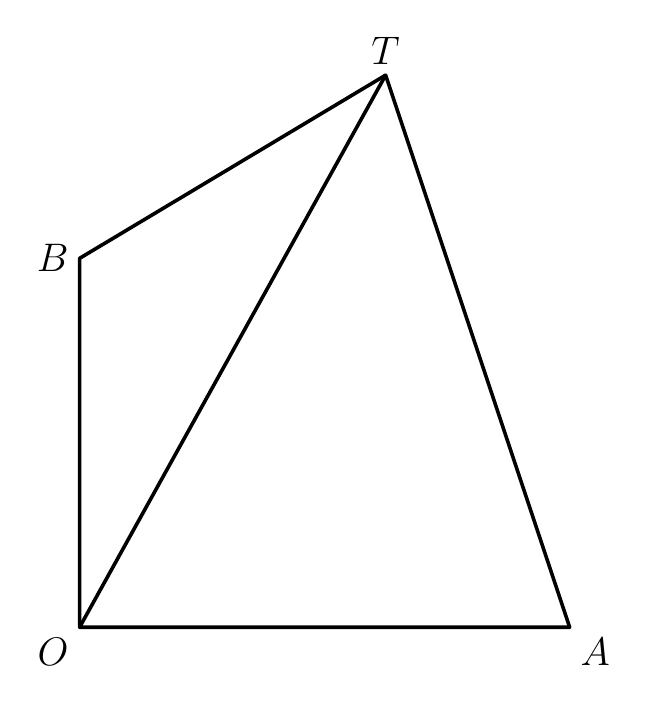
\begin{tikzpicture}[line join=round, line width=1.3pt, font=\fontsize{14}{16.8}\selectfont]
  % Named vertices (converted from pixels; O at origin)
  \coordinate (O) at (0,0);
  \coordinate (A) at (6.224,0);
  \coordinate (T) at (3.887,7.012);
  \coordinate (B) at (0,4.685);

  % Triangle O-A-T and segment O-B-T
  \draw[solid, black] (O) -- (A) -- (T) -- cycle;
  \draw[solid, black] (O) -- (B) -- (T);

  % Labels just outside each vertex
  \node[below left]  at (O) {$O$};
  \node[below right] at (A) {$A$};
  \node[above]       at (T) {$T$};
  \node[left]        at (B) {$B$};
\end{tikzpicture}
\end{document}